\chapter{Appendix I}
\label{sec:appendix}

\section{Detailed Visual Comparison of different Super-Resolution models at UV Texture $256 \rightarrow 512$ task}

\begin{figure}[ht]
	\centering
	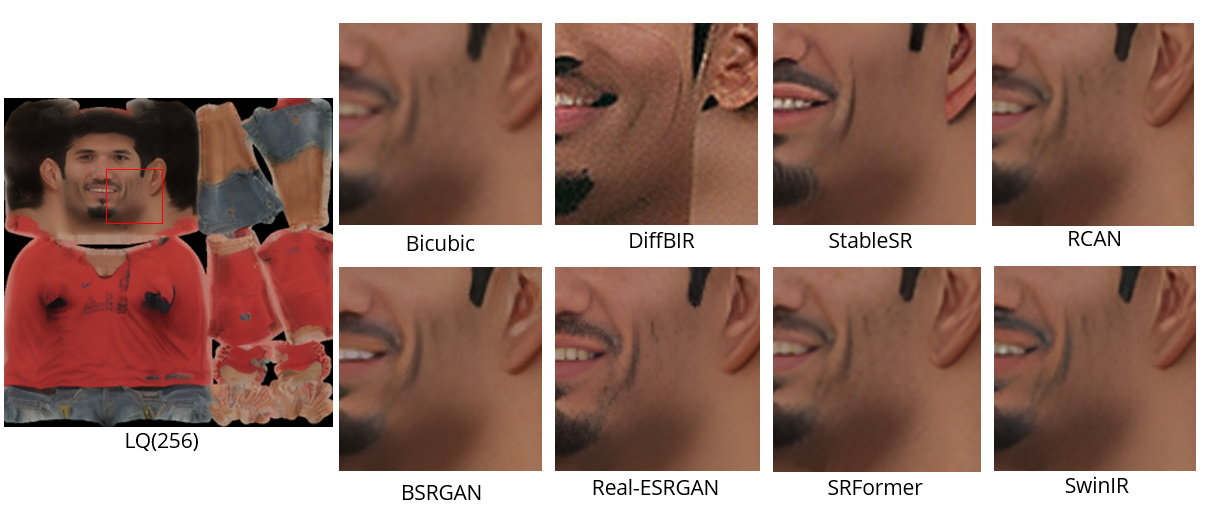
\includegraphics[width=0.9\textwidth]{fig/srface.png}
	\caption{Face detail super-resolution comparison, dataset from SMPLitex.}
	\label{fig:srface}
\end{figure}

\begin{figure}[ht]
	\centering
	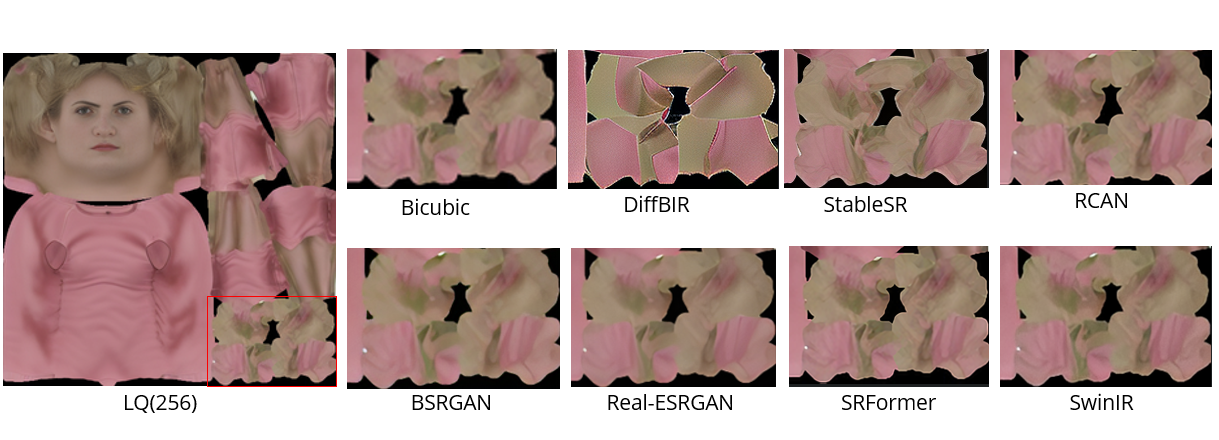
\includegraphics[width=0.9\textwidth]{fig/srhand.png}
	\caption{Hand, foot detail super-resolution comparison, dataset from SMPLitex.}
	\label{fig:srhand}
\end{figure}

\begin{figure}[ht]
	\centering
	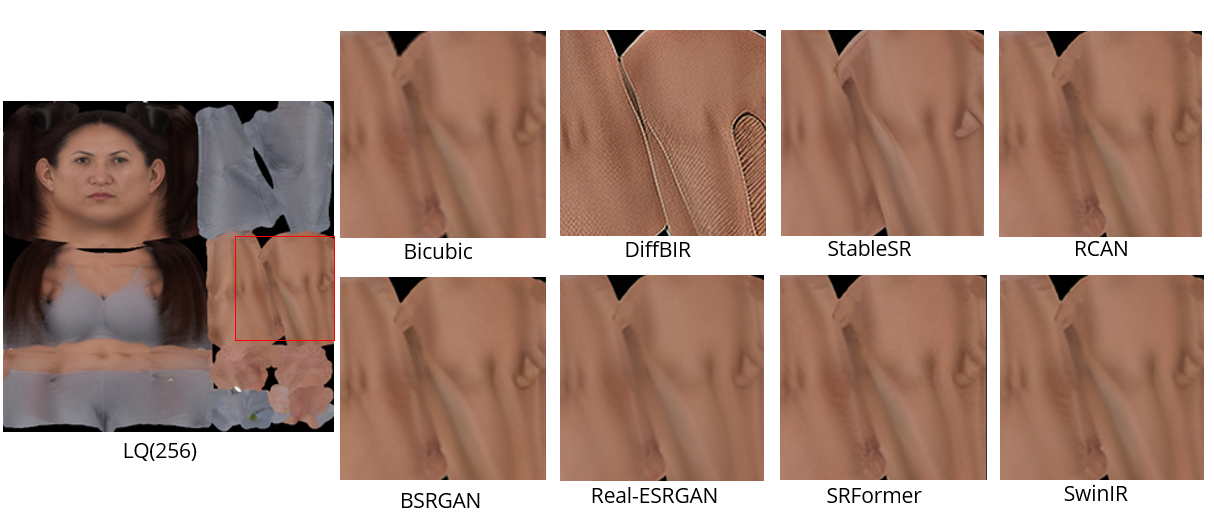
\includegraphics[width=0.9\textwidth]{fig/srmuscles.png}
	\caption{Muscle detail super-resolution comparison, dataset from SMPLitex.}
	\label{fig:srhand}
\end{figure}

\begin{figure}[ht]
	\centering
	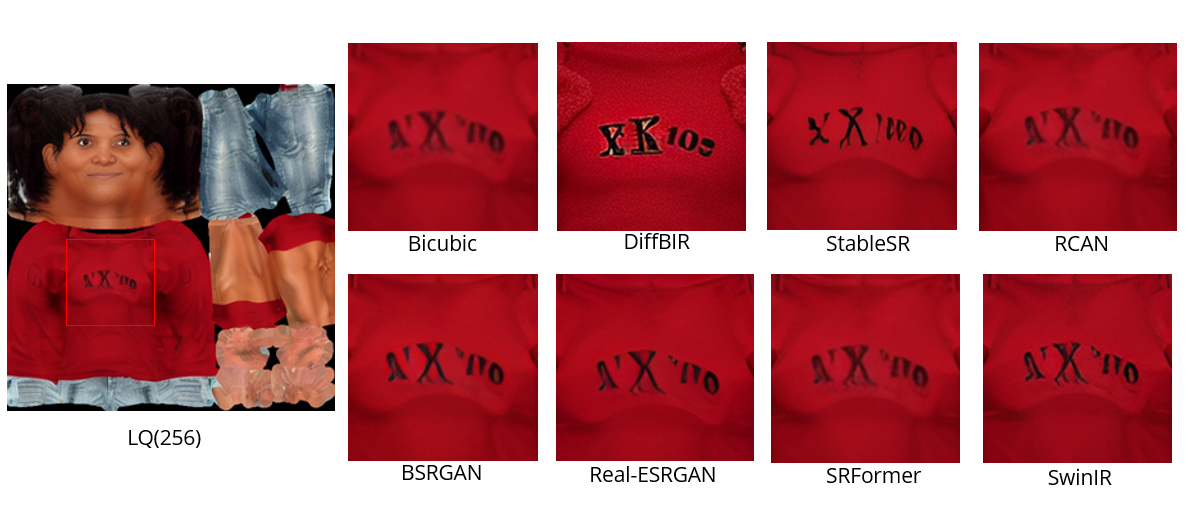
\includegraphics[width=0.9\textwidth]{fig/srcloth.png}
    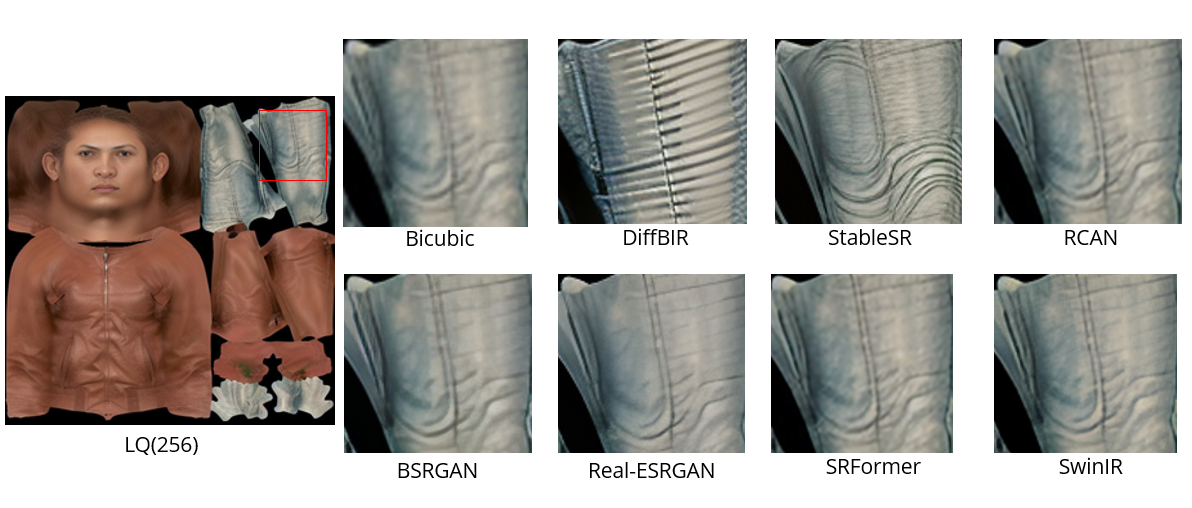
\includegraphics[width=0.9\textwidth]{fig/srcloth2.png}
	\caption{Clothes detail super-resolution comparison, dataset from SMPLitex.}
	\label{fig:srcloth}
\end{figure}



\section{Detailed Visual Comparison of different Super-Resolution models at UV Texture $512 \rightarrow 1024$ task}

\begin{figure}[ht]
	\centering
	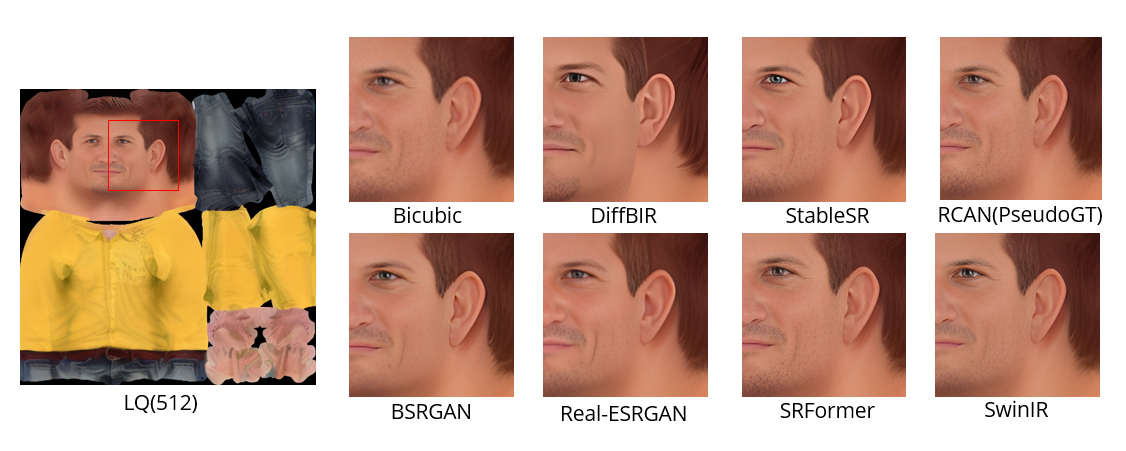
\includegraphics[width=1.0\textwidth]{fig/10241.png}
    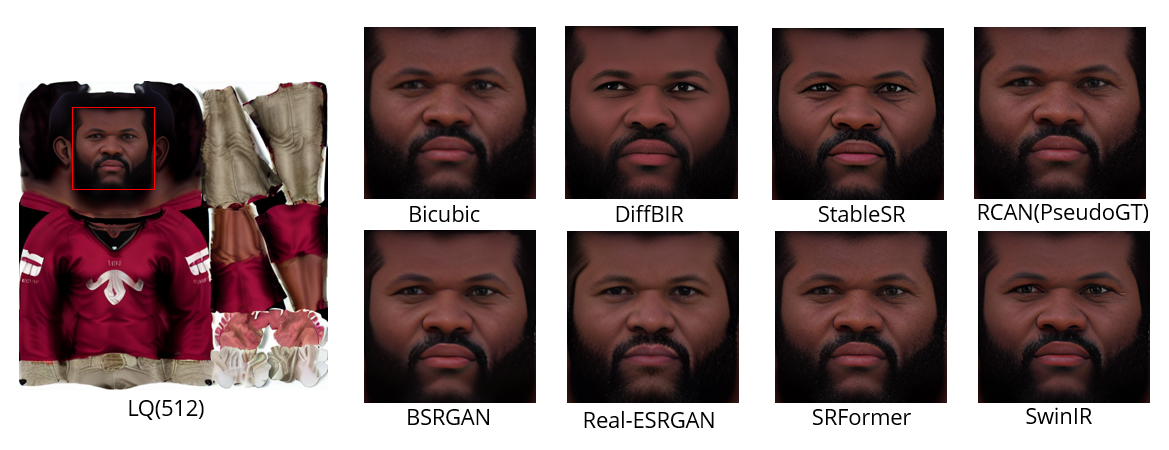
\includegraphics[width=1.0\textwidth]{fig/10242.png}
	\caption{Face detail super-resolution comparison, dataset from SMPLitex.}
	\label{fig:srhand}
\end{figure}

\begin{figure}[ht]
	\centering
	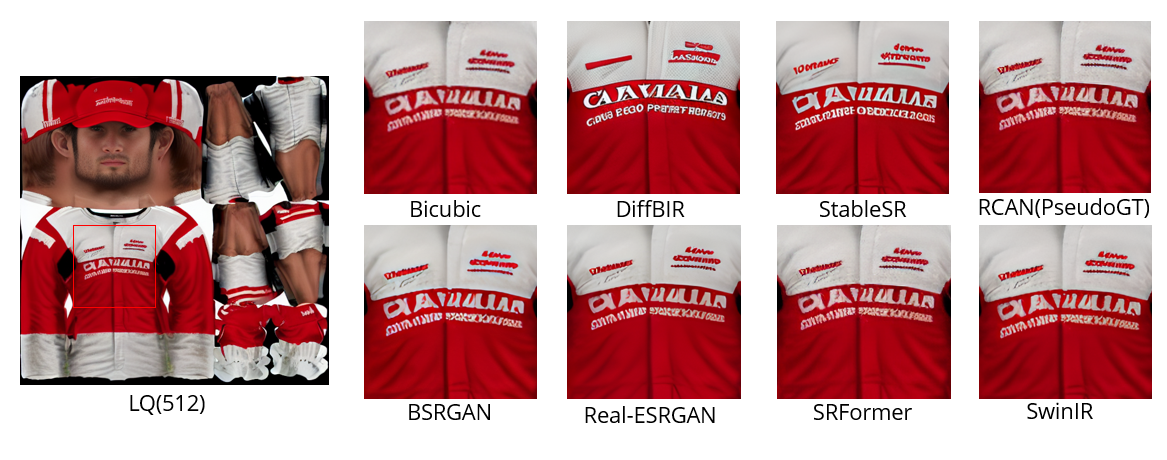
\includegraphics[width=1.0\textwidth]{fig/10243.png}
    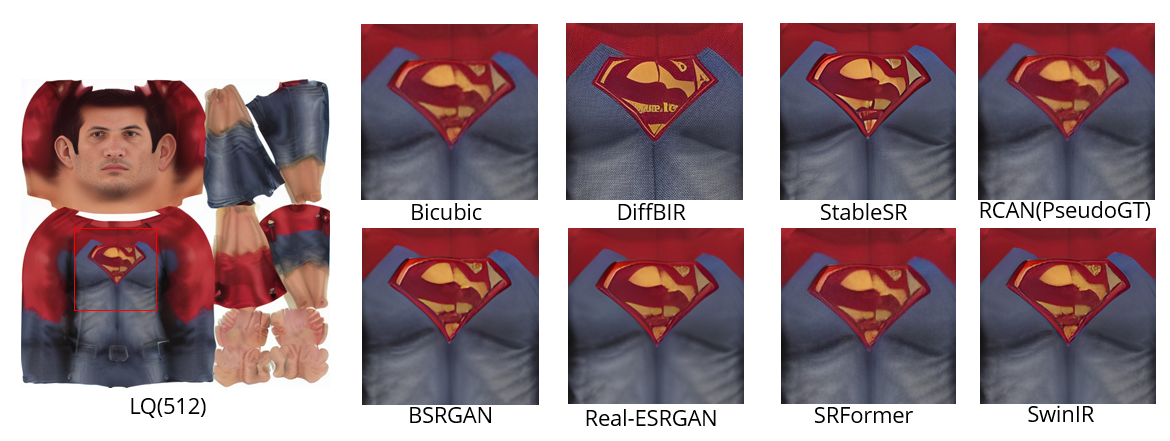
\includegraphics[width=1.0\textwidth]{fig/10244.png}
    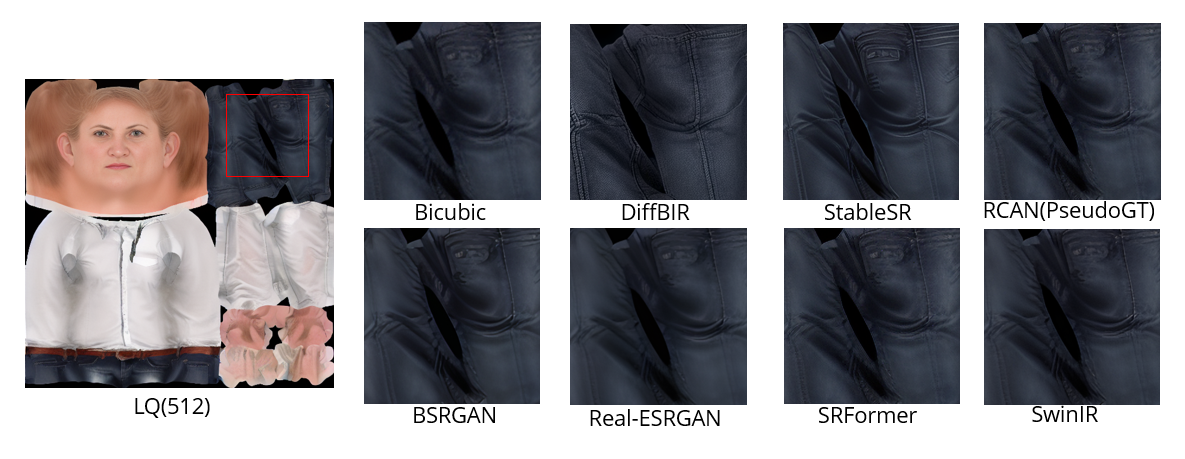
\includegraphics[width=1.0\textwidth]{fig/10245.png}
	\caption{Clothes detail super-resolution comparison, dataset from SMPLitex.}
	\label{fig:srhand}
\end{figure}

\section{Observation on Diffusion-Based SR Models.}
In this appendix, I include a detailed visual comparison of super-resolution models for both $256{\rightarrow}512$ and $512{\rightarrow}1024$ upscaling. These comparisons highlight the importance of texture-level distinctions. More precisely, diffusion-based models such as DiffBIR and StableSR tend to introduce rich high-frequency details. In particular, DiffBIR often adds significant texture complexity--sometimes excessively so.

For example, in the facial regions~\ref{fig:srface}, DiffBIR may produce overdrawn features that deviate from the original identity, a common artifact in diffusion-based synthesis. However, on clothing regions~\ref{fig:srcloth}, DiffBIR consistently enhances fine-scale texture details such as fabric structure, logos, or subtle patterns that are absent or overly smoothed in other SR outputs. This strength in hallucinating plausible garment textures makes DiffBIR-based textures especially valuable for downstream tasks where perceptual richness matters more than pixel-wise fidelity.

This difference explains why the inpainting models trained on the DiffBIR-augmented dataset tend to score poorly under traditional UV-based metrics, such as PSNR, SSIM , LPIPS, and FID in UV space, but achieve superior performance under rendering-based evaluation. The additional detail provided by DiffBIR improves the final appearance once the textures are rendered on the 3D body, even though it diverges from the low-resolution ground truth. This highlights the importance of considering both perceptual and geometric evaluation metrics when assessing texture quality for 3D reconstruction tasks.


\chapter{Appendix II}
\label{sec:appendix2}
\section{Selected Special Cases in Single Image Texture Estimation: A Challenge}
As I mentioned previously, HRHumanTex has certain limitations. For example, when the character's face is not facing the camera, or when the character's upper body clothing texture has complex patterns, it is often impossible to reconstruct a continuous facial texture well and reconstruct the correct leg clothing texture. I refer to these difficult texture estimation problems as a challenge and partially summarize them in this appendix.


\begin{figure}[ht]
	\centering
    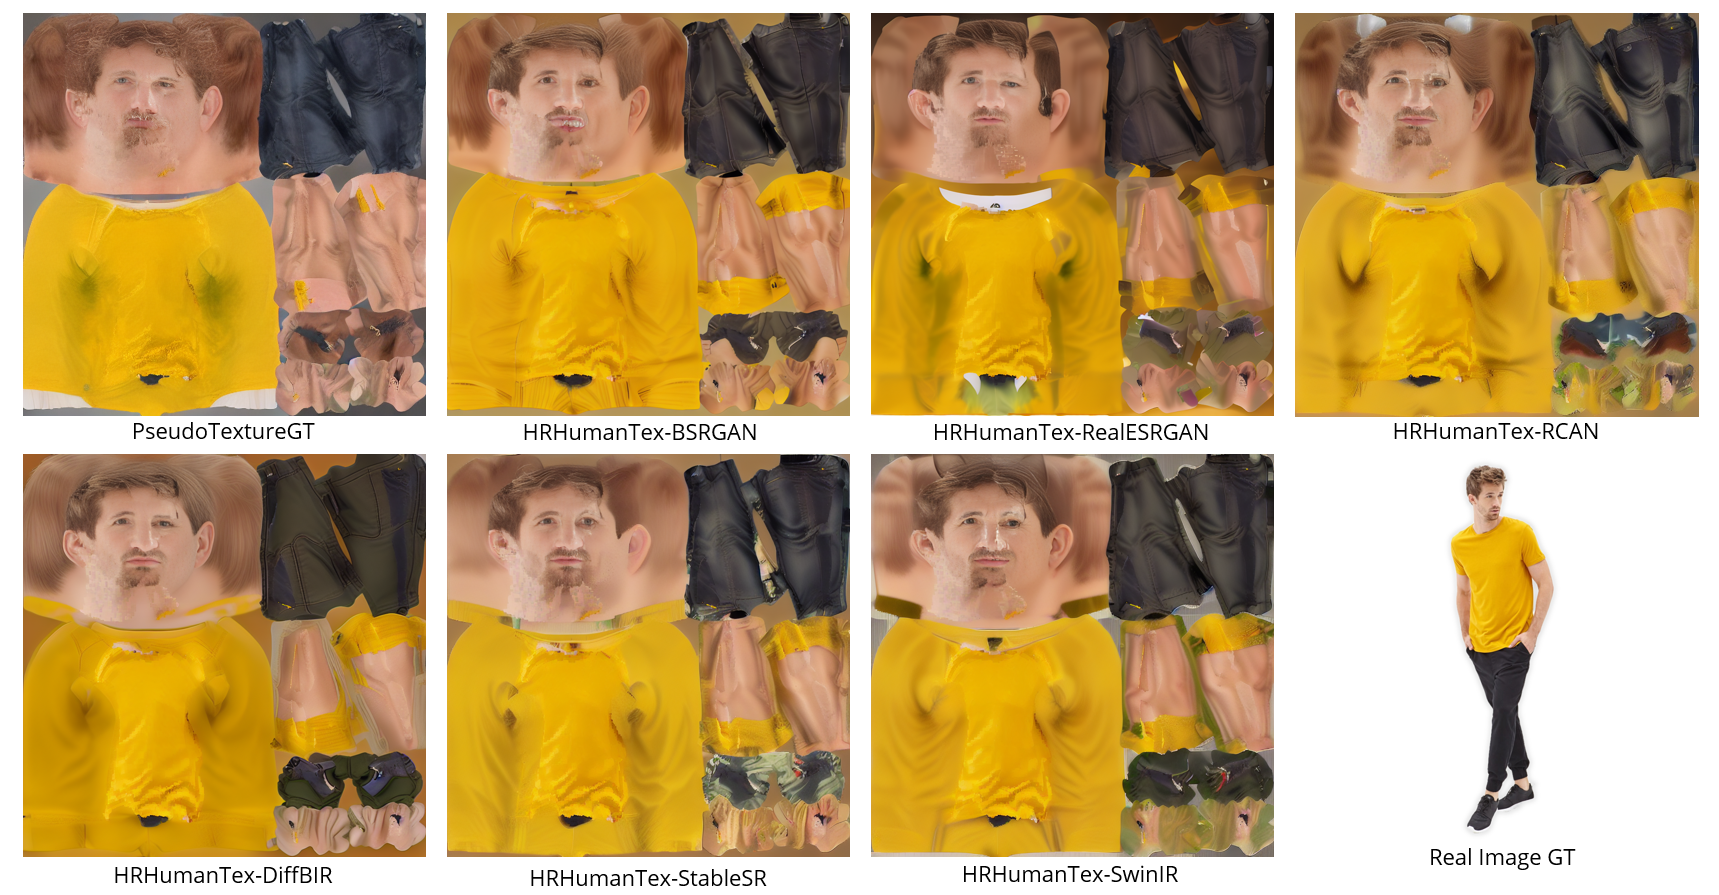
\includegraphics[width=1.0\textwidth]{fig/special1.png}
	\caption{\textbf{Challenge 1: Non-frontal Faces.} When the human is not facing directly to the camera, only \textbf{HRHumanTex-DiffBIR}, \textbf{HRHumanTex-StableSR}, and \textbf{HRHumanTex-SwinIR} manage to reconstruct relatively coherent textures. Other variants failed to preserve structural consistency.}
	\label{fig:sp1}
\end{figure}

\begin{figure}[ht]
	\centering
    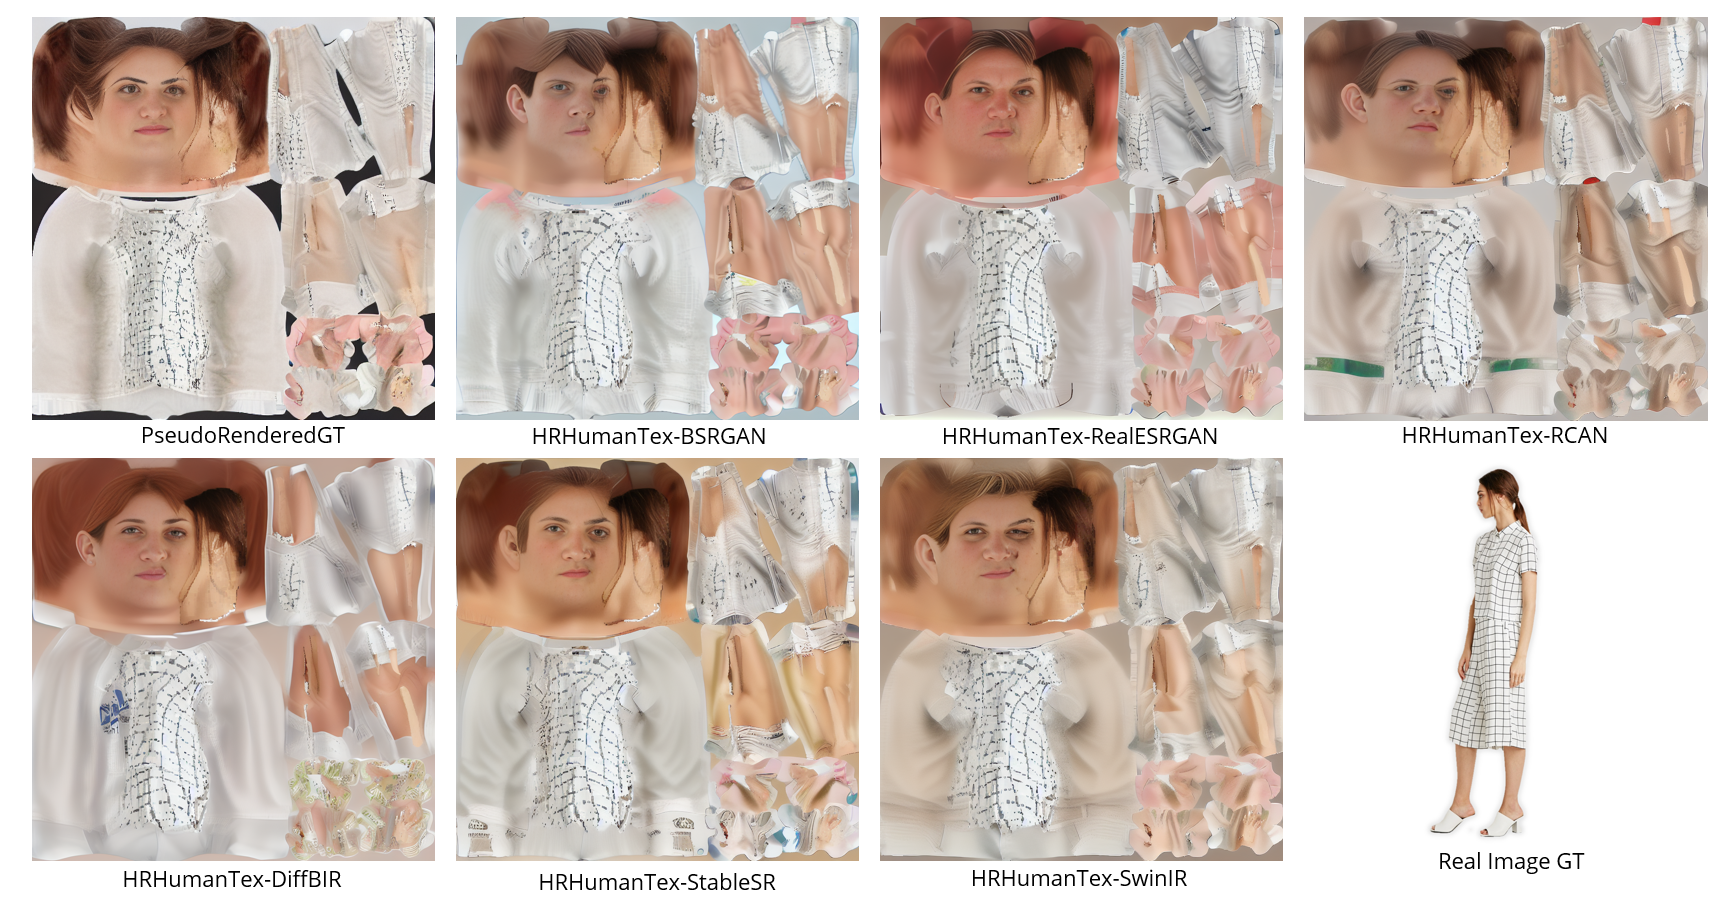
\includegraphics[width=1.0\textwidth]{fig/special2.png}
	\caption{\textbf{Challenge 2: Side Faces.} In cases where the face is not clearly visible or partially occluded, only the \textbf{SMPLitex baseline}, \textbf{HRHumanTex-DiffBIR}, and \textbf{HRHumanTex-StableSR} were able to hallucinate a plausible face texture. All other models incorrectly generated masculine features from a clearly female subject.}
	\label{fig:sp2}
\end{figure}

\begin{figure}[ht]
	\centering
    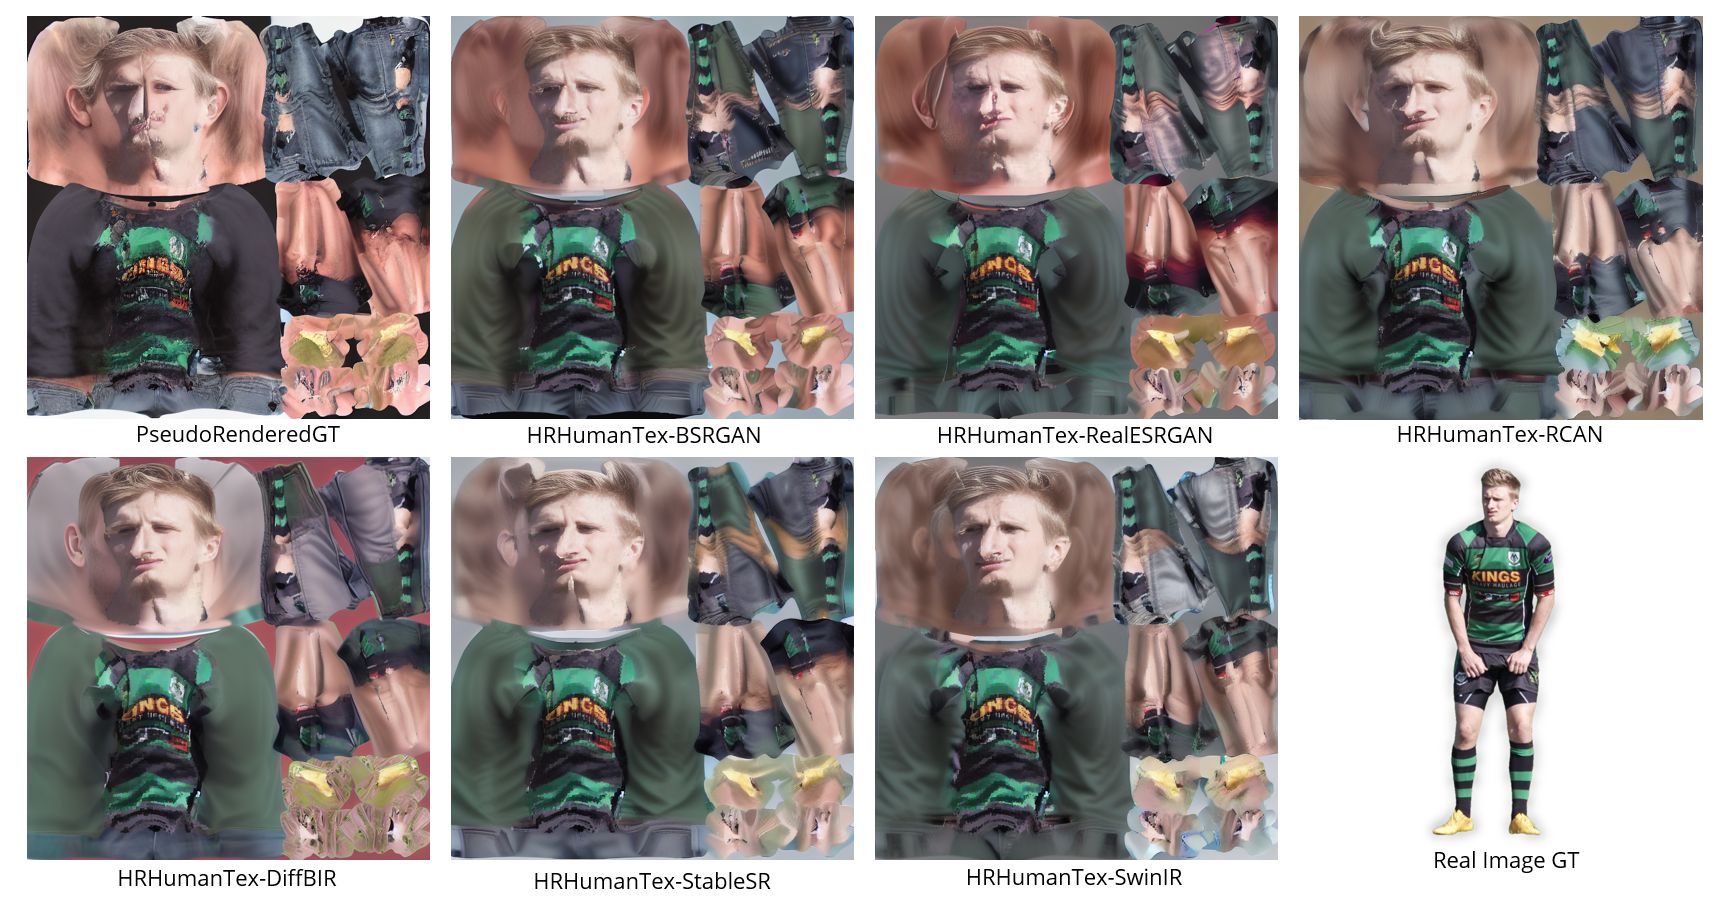
\includegraphics[width=1.0\textwidth]{fig/special3.png}
	\caption{\textbf{Challenge 3: Non-frontal Faces.} Only HRHumanTex-DiffBIR, HRHumanTex-StableSR, and HRHumanTex-SwinIR reconstructed coherent textures compared to other models, but the textures were not clear enough. Other models failed.}
	\label{fig:sp3}
\end{figure}

\begin{figure}[ht]
	\centering
    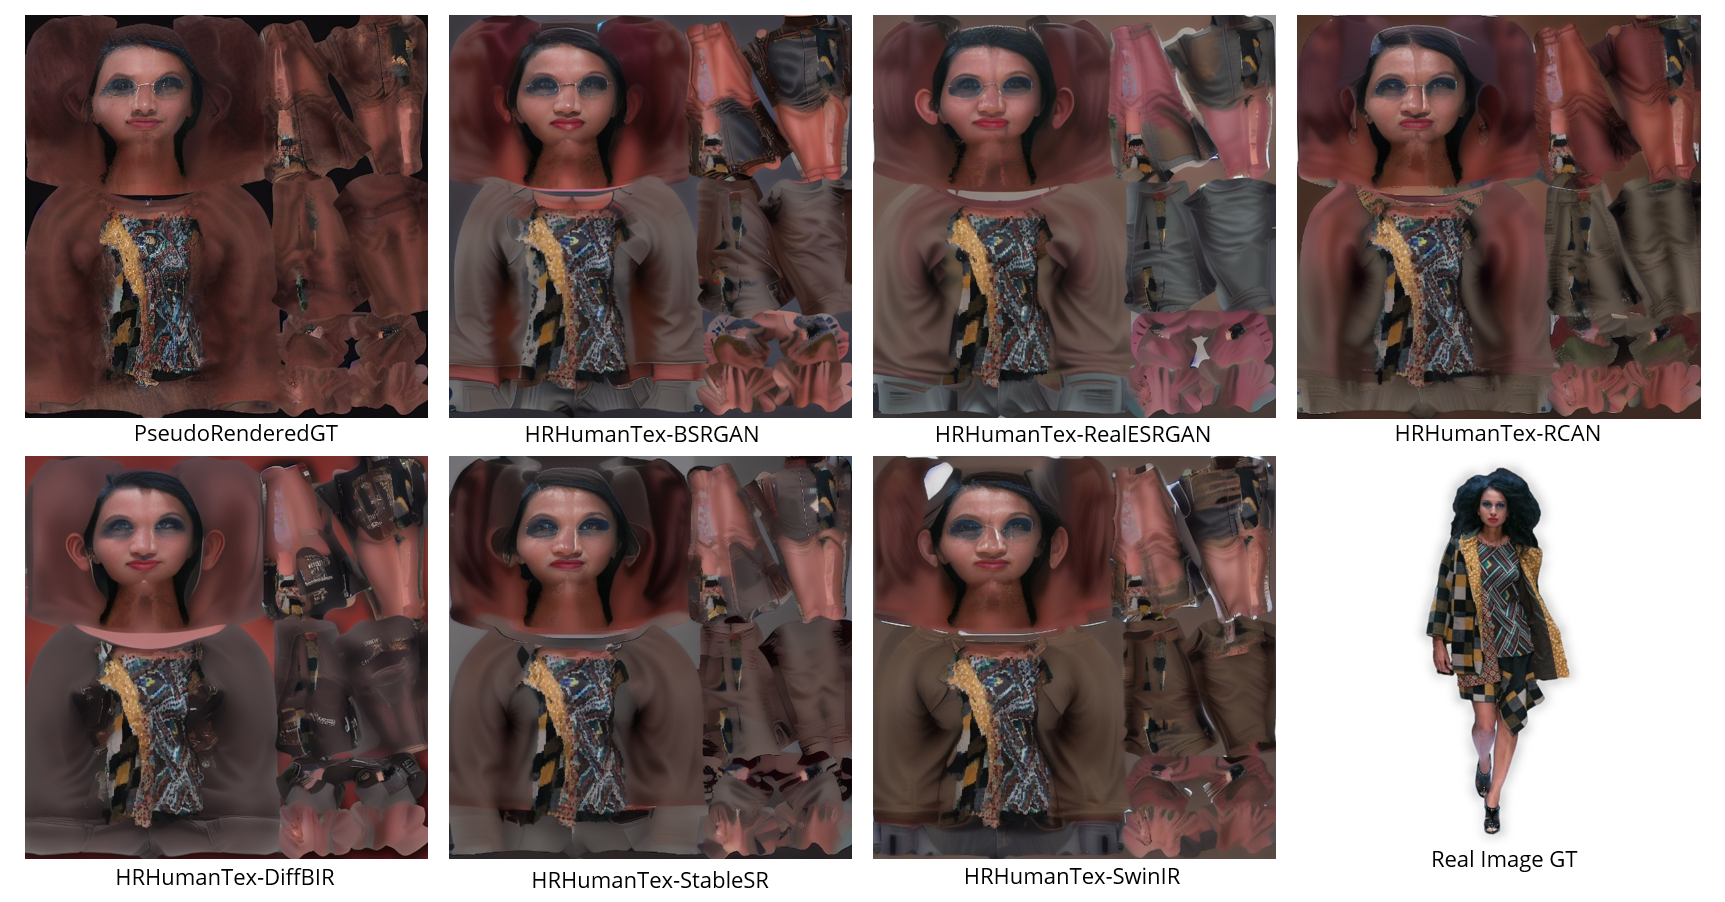
\includegraphics[width=1.0\textwidth]{fig/special4.png}
	\caption{\textbf{Challenge 4: Makeup Confusion.} In one example, only \textbf{HRHumanTex-DiffBIR} successfully reconstructed the subject’s heavy eye makeup (smoky eyes), while all other models mistakenly rendered dark sunglasses, possibly due to texture prior bias.}
	\label{fig:sp4}
\end{figure}

\begin{figure}[ht]
	\centering
    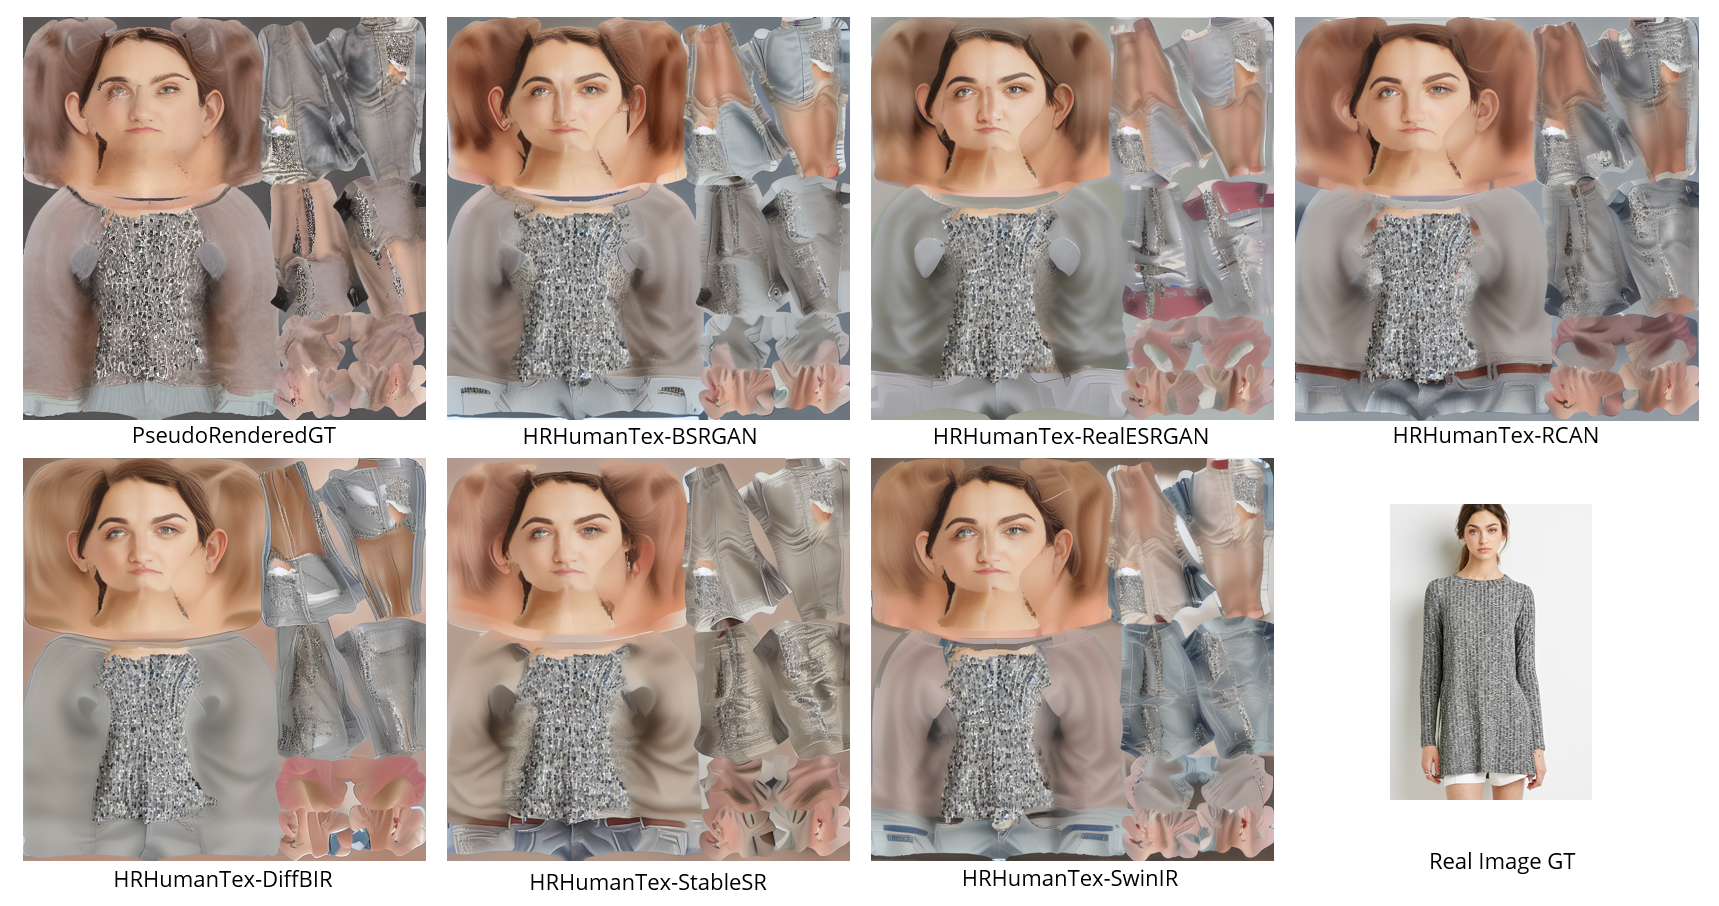
\includegraphics[width=1.0\textwidth]{fig/special5.png}
	\caption{\textbf{Challenge 5: Garment Length Interference.} When the upper garment occludes the lower body, all models failed to reconstruct the white shorts worn by the subject. Instead, they wrongly extended the denim texture of the top garment downwards, demonstrating a limitation in body-part disambiguation.}
	\label{fig:sp5}
\end{figure}

\begin{figure}[ht]
	\centering
    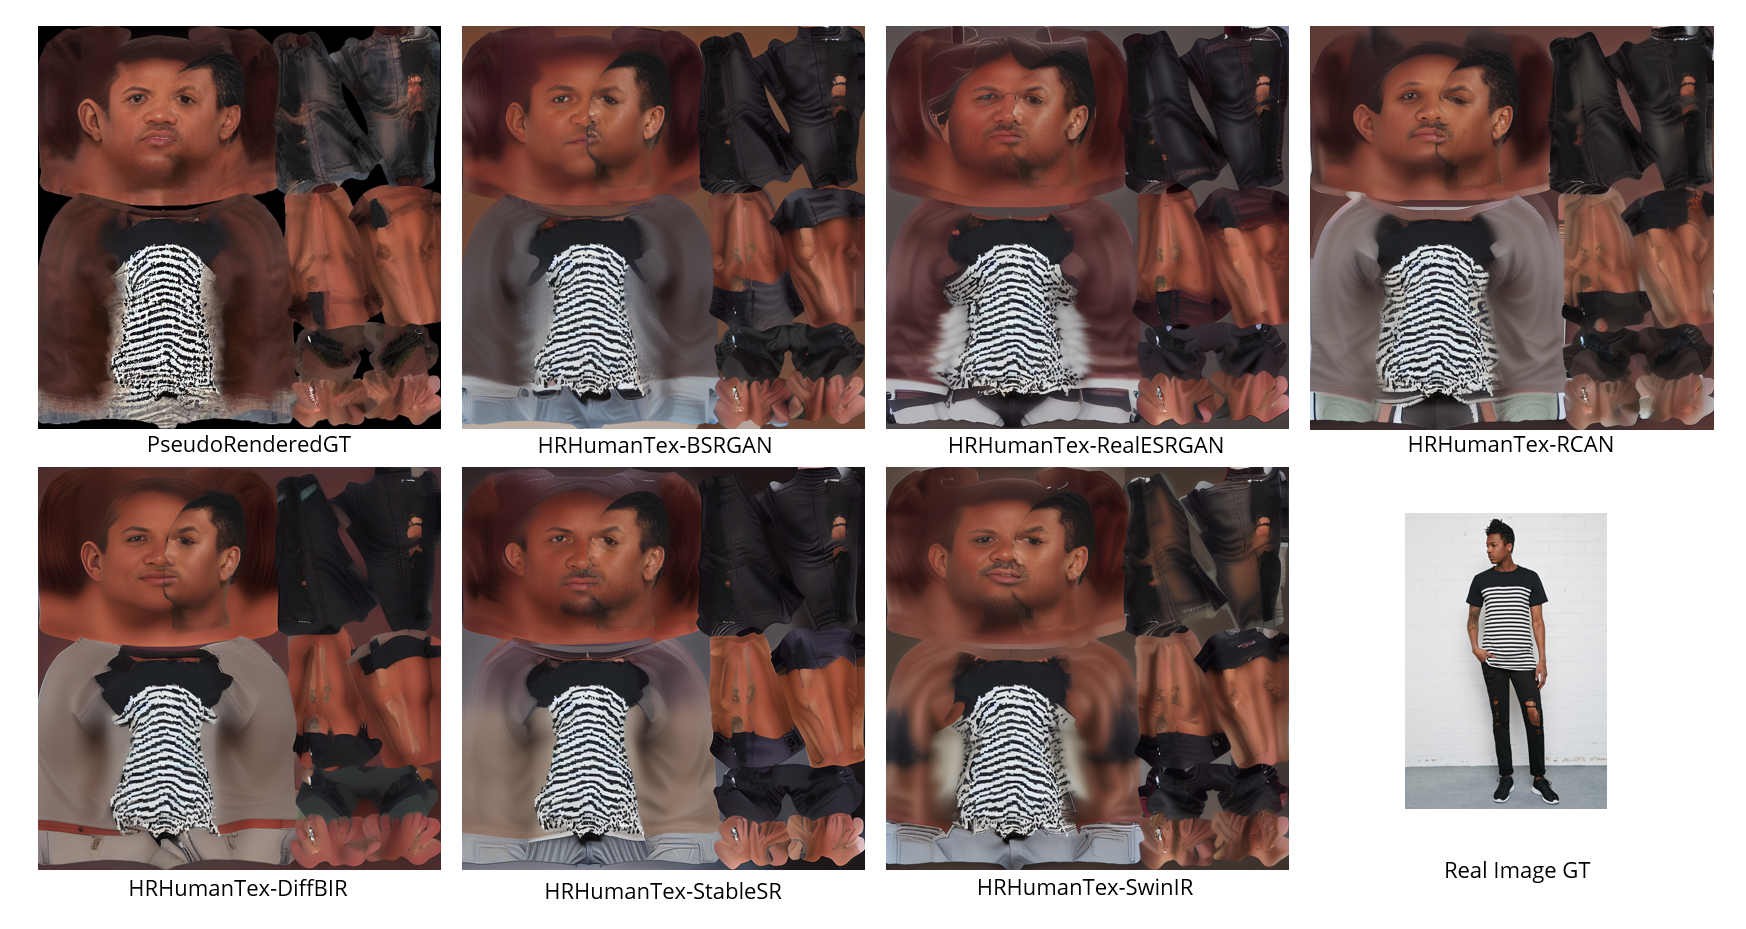
\includegraphics[width=1.0\textwidth]{fig/special6.png}
	\caption{\textbf{Challenge 6: Side Faces.} Since the human was facing the camera sideways, all models were unable to successfully reconstruct the facial texture of the human and all failed.}
	\label{fig:sp6}
\end{figure}

While my main quantitative analysis in the main paper highlights \textbf{HRHumanTex-DiffBIR} and \textbf{HRHumanTex-SwinIR} as the overall best-performing models, the qualitative observations from these challenging cases suggest that \textbf{HRHumanTex-DiffBIR} may offer superior robustness in difficult scenarios. In particular, its ability to hallucinate plausible textures under occlusion, low visibility, or stylistic ambiguity (e.g., makeup or skin tone) makes it a strong candidate for practical deployment in real-world applications.

\chapter{Appendix III}
\label{sec:appendix3}

\section{Additional implementation detail.}
To complete the UV texture from partial observations, I employed the \texttt{img2img} interface from my internal \texttt{sd\_api}, which is based on Stable Diffusion. The interface supports multi-sample generation by specifying a \texttt{batch\_size}. In my implementation, I set \texttt{batch\_size = 8} to produce diverse texture candidates per input. Among the 8 outputs, I manually selected the most visually plausible result based on detail continuity and garment identity preservation. Because there are always some particularly good and some particularly bad candidates among the 8 candidates, it is relatively easy to screen them with the naked eye.

The Python snippet below shows the actual inpainting call:

\begin{figure}[ht]
	\begin{lstlisting}[language=Python]
# inpaints input image (note: generates 8 versions)
inpainted_result = self.sd_api.img2img(
    "a sks texturemap", 
    images=[im], 
    batch_size=8,
    mask_image=im_mask, 
    cfg_scale=cfg,
    denoising_strength=denoising_strength,
    restore_faces=True,
    width=1024,
    height=1024,
)
	\end{lstlisting}
	\caption{Code used for texture inpainting via Stable Diffusion.}
	\label{code:inpaint_api}
\end{figure}

To ensure secure and reproducible execution of the inpainting pipeline, I installed Stable Diffusion on a dedicated user account with appropriate file permissions. The setup procedure was as follows:

\begin{itemize}
\item \textbf{Create and activate a Python virtual environment}:
\begin{lstlisting}[language=bash]
python3.10 -m venv venv
source venv/bin/activate
\end{lstlisting}
\item \textbf{Create a new user and assign permissions to working directory}:
\begin{lstlisting}[language=bash]
adduser sduser
chown -R sduser:sduser /workspace/
su - sduser
\end{lstlisting}
\item \textbf{Activate the environment and launch web interface}:
\begin{lstlisting}[language=bash]
cd /workspace/stable-diffusion-webui
source venv/bin/activate
./webui.sh --disable-safe-unpickle --api
\end{lstlisting}
\end{itemize}


To allow external access and remote API usage, I modified the webui.py script to explicitly expose the server with the following arguments: share=True and server\_name="0.0.0.0". The edited shared.demo.launch 
 call is shown below:

\begin{figure}[ht]
\begin{lstlisting}[language=Python]
app, local_url, share_url = shared.demo.launch(
share=True,
server_name="0.0.0.0",
server_port=7860,
ssl_keyfile=cmd_opts.tls_keyfile,
ssl_certfile=cmd_opts.tls_certfile,
ssl_verify=cmd_opts.disable_tls_verify,
debug=cmd_opts.gradio_debug,
auth=gradio_auth_creds,
inbrowser=auto_launch_browser,
prevent_thread_lock=True,
allowed_paths=cmd_opts.gradio_allowed_path,
app_kwargs={"docs_url": "/docs", "redoc_url": "/redoc"},
root_path=f"/{cmd_opts.subpath}" if cmd_opts.subpath else "",
)
\end{lstlisting}
\caption{Modified Gradio launch call in \texttt{webui.py} to support remote access.}
\end{figure}

\chapter{Appendix IIII}
\label{sec:appendix4}
\section{Acknowledgements}

Firstly, I would like to thank my supervisor Dr.Kristijan Bartol, and Prof. Stefan Gumhold, for their insightful guidance and continuous support throughout the development of this thesis.  Whether it was the discussion with Professor Gumhold or the email communication with Dr. Bartol, they all inspired me to keep moving forward. Sincerely appreciate their support!

I would like to express my deepest gratitude to my parents, who have always supported me unconditionally, even from afar in China. In particular, I am profoundly grateful to my father, whose financial support made it possible for me to conduct experiments using the high-performance RTX 3090 24GB GPU. Thanks for my mother and father's support, I could have a chance to study abord at Germany, especially at excellent TU Dresden in Die schönste Stadt Dresden.

I also wish to thank the RunPod platform and Google Colab for providing accessible and user-friendly cloud GPU services, which have greatly empowered independent researchers and students like myself to explore ambitious research topics.

Last but not least, I want to thank my girlfriend, Chuyi, my beloved cat，Haidai. During countless late nights of debugging and failed experiments, Haidai’s innocent eyes always brought me calm and joy, and Chuyi’s constant encouragement reminded me to persevere and keep going. I sincerely wish Chuyi all the best in her computer studies at TU Darmstadt. Their companionship made this challenging journey warm and meaningful.
